\chapter{Úvod}

Strojové učenie predstavuje ďalší logický krok v počítačovej vede. Programovanie
založené na pevne danom správaní prestáva pre mnohé úlohy stačiť. Na softvérové
produkty sú kladené čoraz väčšie nároky, a v dohĺadnej dobe sa dá očakávať
dosihanutie hranice tradičného prístupu. Dôvodom je najmä veľmi rozsiahly stavový priestor úloh.
Možným východiskom sú adaptíve a učiace sa systémy.

\section{Markovove rozhodovacie procesy}

Množstvo úloh je možné popísať množinou stavou $\mathbb{S}$, pre každý stav je definovaná množina akcií
$\mathbb{A_S}$. Pre každý stav a každú akciu, ktorú je v ňom možné vykonať existuje pravedepodobnostná
funkcia prechodu do ďalšieho stavu $P(s, s')$ a za uskutočnené prechody je daná funkcia odmien $R(s, s')$.
Formálne je teda Markovov proces pätica $(\mathbb{S}, \mathbb{A_S}, P(s, s'), R(s, s'), \gamma )$,
kde $\gamma \in (0, 1)$ je faktor zabúdania, a volí sa ako parameter procesu. Jeho význam bude vysvetlený
v ďalšej kapitole. Príklad Markovovho rozhodovacieho procesu je na obrázku \ref{img:markovov_decision_process}.
Prechody v grafe znamenajú jednotlivé akcie.

\begin{figure}[!htb]
\center
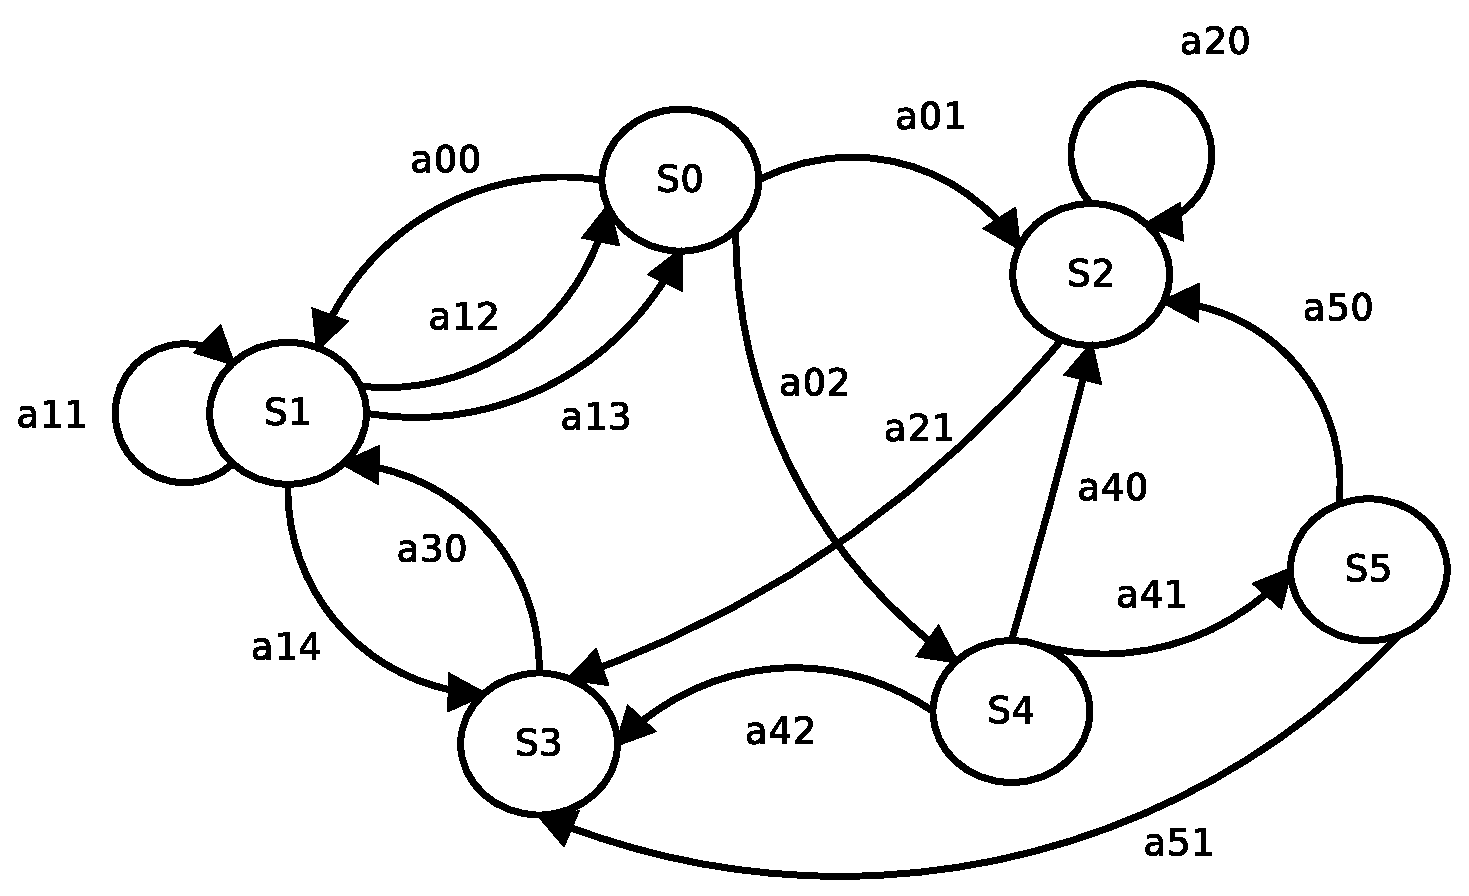
\includegraphics[scale=.5]{../diagrams/markovov_process.eps}
\caption{Markovov rozhodovací proces}
\label{img:markovov_decision_process}
\end{figure}

V priestore stavov $\mathbb{S}$ existuje výkonná jednotka - agent. Je to modul
ktorý na základe vstupnej informácie - stave vyberie jednu z akcií. To s akou pravdepodobnosťou
sa daná akcia vykoná je dané prostredím (popísané Markovove rozhodovacím procesom).

Dôležitým východiskom je, že $P(s, s')$ nie je agentovi známa. Agent teda nemôže
vedieť kam sa vykonaním vybranej akcie dostane. Tento fakt značne komplikuje prehľadávanie
priestoru.
Ďalším typickým rysom je, že odmeňovacia funkcia $R(s, s')$, ktorá je zadaná,
nadobúda pre väčšinu prechodov z $s$ do $s'$ hodnotu 0. Je to dôsledok prirodzeného
spôsobu riešenia problémov delením na čiastkové kroky a nie je okamžite známa
veľkosť úžitku po vykonaní čiastkového kroku. Často je táto skutočnosť známa
len pre pár vybraných prechodov.
Dobrým príkladom tejto situácie je hra Go.

\begin{figure}[!htb]
\center
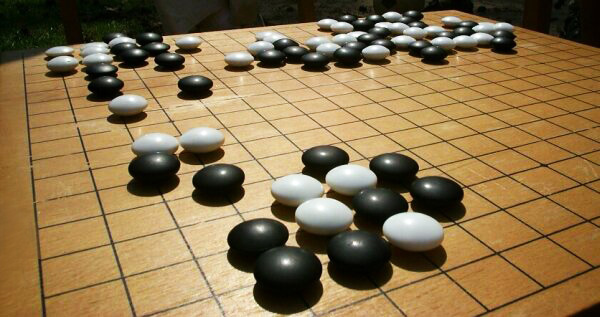
\includegraphics[scale=.5]{../pictures/go2.jpg}
\caption{Hra Go}
\label{img:go_game}
\end{figure}

Položením kameňa na Goban nie okamžite známe ako to ovplyvní priebeh hry.
Je bežné, že sa to prejaví až po mnohých krokoch.
